%Estudiar con cuidado. Aquí va el corazón: enunciar ETH (diagonal/off-diagonal), suavidad en energía, implicaciones para observables locales.
%1 slide con la fórmula ETH y un diagrama explicando “ventana microcanónica”.

\begin{frame}
\frametitle{Ansatz of ETH}

\begin{block}{Ansatz equation}
ETH can be formulated as an ansatz for the matrix elements of observables in the basis
of the eigenstates of a Hamiltonian 
\begin{equation}
O_{mn} = O(\bar{E})\,\delta_{mn} + e^{-S(\bar{E})/2} f_{O}(\bar{E}, \omega)\, R_{mn},
\end{equation}

\end{block}

\begin{block}{Microcanonical limit}
\begin{equation}
\overline{O} \equiv \lim_{t_0 \to \infty} \frac{1}{t_0} \int_{0}^{t_0} dt\, O(t)
= \sum_m |C_m|^2 O_{mm} = \mathrm{Tr}\!\left[\hat{\rho}_{\mathrm{DE}} \hat{O}\right],
\end{equation}

\begin{equation}
O_{\mathrm{ME}} = \mathrm{Tr}\!\left[\hat{\rho}_{\mathrm{ME}} \hat{O}\right],
\end{equation}

\begin{equation}
\overline{O} \simeq O(\langle E \rangle) \simeq O_{\mathrm{ME}}.
\end{equation}

\end{block}
\end{frame}

\begin{frame}{Microcanonical window example}
\begin{block}{One-dimensional periodic chains of interacting spinless fermions hamiltonian operator}
\begin{equation}
\begin{split}
\hat{H} = \sum_{j=1}^{L} \Bigg[
    &-J \left( \hat{b}_j^{\dagger} \hat{b}_{j+1} + \text{H.c.} \right)
    + V \left( \hat{n}_j - \frac{1}{2} \right)
      \left( \hat{n}_{j+1} - \frac{1}{2} \right) \\
    &- J' \left( \hat{b}_j^{\dagger} \hat{b}_{j+2} + \text{H.c.} \right)
    + V' \left( \hat{n}_j - \frac{1}{2} \right)
      \left( \hat{n}_{j+2} - \frac{1}{2} \right)
\Bigg].
\end{split}
\end{equation}
\end{block}
\end{frame}

\begin{frame}{Microcanonical window example}
\begin{block}{Zero momentum mode occupation operator}
\begin{equation}
\hat{m}(k) = \frac{1}{L} \sum_{i,j} e^{ik(i-j)} \hat{b}_i^{\dagger} \hat{b}_j .
\end{equation}
\end{block}

\begin{block}{Kinetic energy per site operator}
\begin{equation}
\begin{split}
\hat{K} = \frac{1}{L} \sum_{j=1}^{L} \Big[
    -J \left( \hat{b}_j^{\dagger} \hat{b}_{j+1} + \text{H.c.} \right)
    - J' \left( \hat{b}_j^{\dagger} \hat{b}_{j+2} + \text{H.c.} \right)
\Big].
\end{split}
\end{equation}
\end{block}

\end{frame}


\begin{frame}{Microcanonical window example and diagonal elements}
\begin{figure}
    \centering
    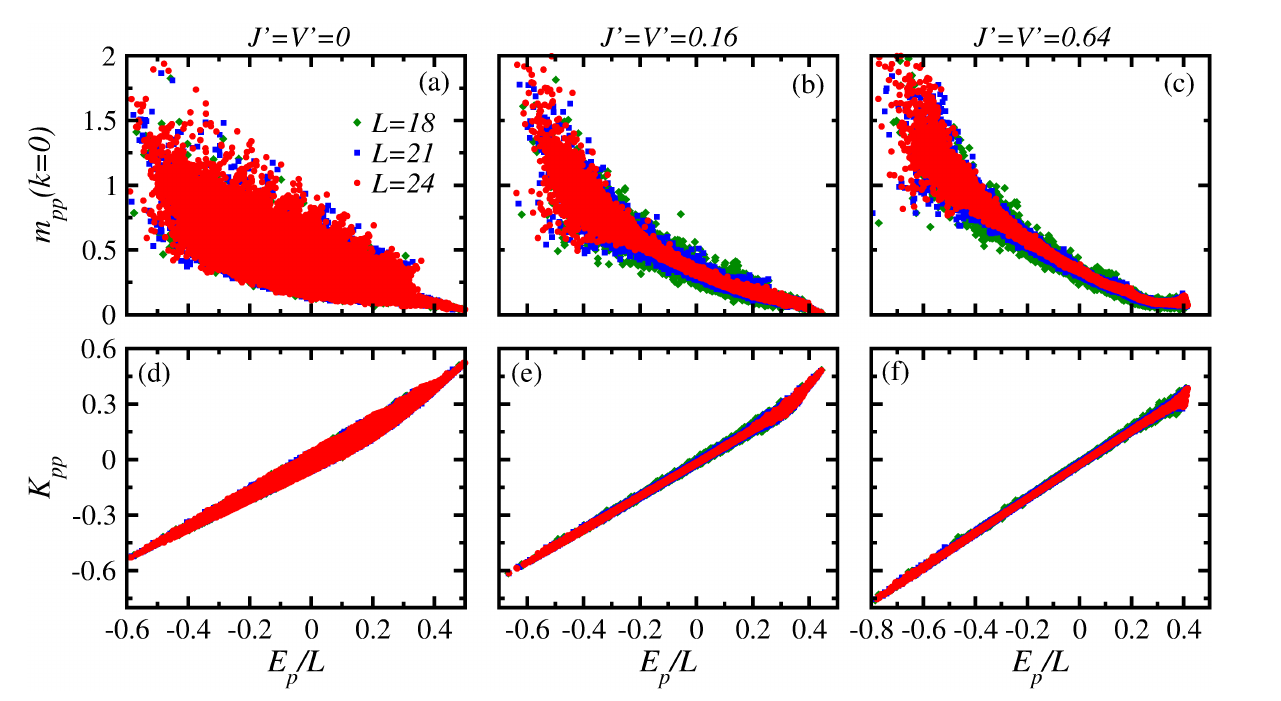
\includegraphics[width=\textwidth]{microcanonical-window.png}
    \caption{Eigenstate expectation values of the occupation of the zero momentum mode [(a)–(c)] and the kinetic
energy per site [(d)–(f)] of hard-core.}
\end{figure}
\end{frame}

\begin{frame}{Microcanonical window example and off-diagonal elements}
\begin{figure}
    \centering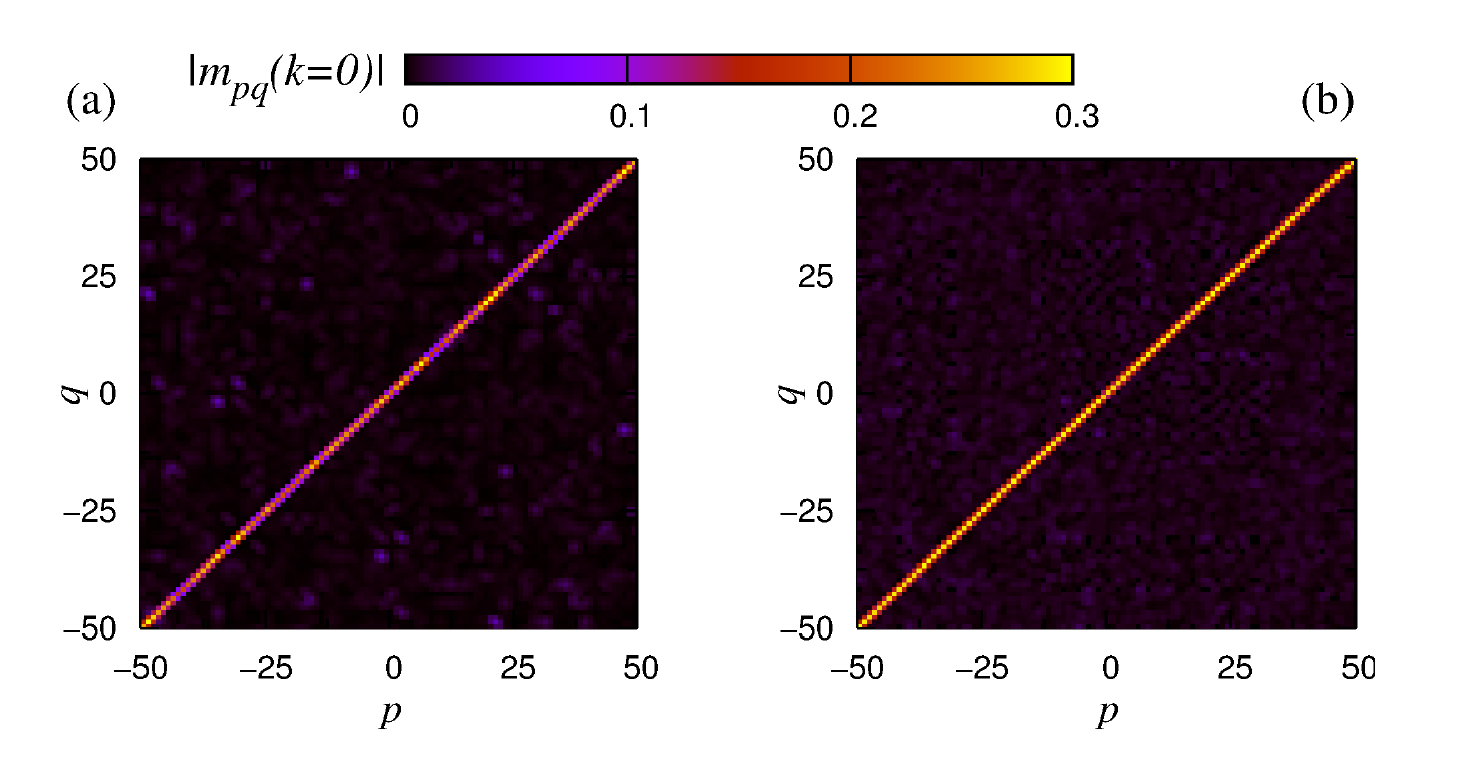
\includegraphics[width=\textwidth]{off-diagonal_matrix.png}
    \caption{Off-diagonal matrix elements of m(k = 0) in the eigenstates of the Hamiltonian.}
\end{figure}

\end{frame}